\documentclass[hidelinks,11pt]{article}

\usepackage[margin=1in]{geometry}
\usepackage{mathpazo}
\usepackage{nicefrac}
\usepackage[title,titletoc,toc]{appendix}
\usepackage{multirow}
% for much better looking tables
\usepackage{booktabs} 
% tables spanning multiple pages
\usepackage{longtable}

%%% FIGURES AND FLOATS
% make it possible to include more than one captioned figure/table in a single float
\usepackage{subcaption} 
\usepackage{graphicx}
% Enables the Here Dammit figure position.
\usepackage{float} 
\usepackage{dblfloatfix}
\usepackage{fixltx2e}
\usepackage[format=plain,font=small,labelfont=bf]{caption} %caption
                                %formatting

%%% MISC
\usepackage[utf8]{inputenc}
\usepackage{blindtext}
\usepackage{cleveref}
\usepackage[hidelinks,bookmarks]{hyperref}

\usepackage{listings} % All code (looks nicer...)
\usepackage{xcolor,color}
\definecolor{mygreen}{rgb}{0,0.6,0}
\definecolor{dkgreen}{rgb}{0,0.6,0}
\definecolor{dkpurple}{rgb}{0.4,0.1,0.4}
\definecolor{blue}{rgb}{0.0,0.0,1.0}
\definecolor{light-gray}{gray}{0.9}
\definecolor{gray}{rgb}{0.5,0.5,0.5}
\definecolor{mauve}{rgb}{0.58,0,0.82}
\definecolor{green}{RGB}{0,127,0}

\lstdefinestyle{java}{ language=Java }
\lstdefinestyle{c}{ language=C }
\lstdefinestyle{python}{ language=Python }
\lstdefinestyle{makefile}{ language=[gnu]make }
\lstdefinestyle{bash}
{
  language=bash,
  backgroundcolor=\color{light-gray}
}

\lstset
{
  numbers=left, 
  firstnumber=1,
  stepnumber=1,
  numberfirstline,
  numberstyle=\scriptsize, %\sffamily
  frame=single, 
  frameround=tttt,
  tabsize=4,
  basicstyle=\small\ttfamily, 
  keywordstyle=\bfseries\color{dkpurple},
  stringstyle=\color{blue}, 
  commentstyle=\color{dkgreen}, 
  showstringspaces=false,
  aboveskip=0.5em, 
  belowskip=0em,
  captionpos=b,
  xleftmargin=1.5em,
  xrightmargin=0.5em
}

\usepackage{MnSymbol}
\lstset{prebreak=\raisebox{0ex}[0ex][0ex]
        {\ensuremath{\rhookswarrow}}}
\lstset{postbreak=\raisebox{0ex}[0ex][0ex]
        {\ensuremath{\rcurvearrowse\space}}}
\lstset{breaklines=true, breakatwhitespace=true}
%%% BIBLIOGRAPHY
\usepackage{cite}


%%% Fancy page style
\usepackage{fancyhdr} % fancy headers
\pagestyle{fancy}
\fancyhead{}

\sloppy
\frenchspacing

\renewcommand{\headrulewidth}{0.4pt}
\renewcommand{\footrulewidth}{0.4pt}
\setlength{\parindent}{0.0in}
\setlength{\parskip}{3pt}

\fancyhead{}
\fancyhead[L]{Project 4 -- Face Recognition}
\fancyhead[R]{Koch, Hart, Beckman}
\fancyfoot{}
\fancyfoot[L]{New Mexico Tech / Fall 2014 / Math 430}
\fancyfoot[R]{\thepage}

\begin{document}
\title{Project 4: Face Recognition}
\author{Christopher Koch\\David Hart\\Darrel Beckman\\
Math 430}
\maketitle

\section{Introduction}
\label{sec:intro}

In this project, we seeked to classify images of faces by gender using machine
learning. This was based on a face database\cite{fei} from the Centro
Universitário da FEI in Brazil, which included both smiling and non-smiling
aligned images. The algorithm developed on these images was then used on 1000
images from the Labeled Faces in the Wild database out of the University of
Massachusetts\cite{lfw}. 

Two classification methods were used: a simple method based on the rank-2
SVD approximation coefficients and an LDA na\"ive Bayes classifier. Both yielded
fairly accurate results.

\section{Model Description}
\label{sec:model}

Several methods of face classification were tried. First, singular values were
obtained for both smiling and non-smiling images and it was clear that they were
approximately in the same range. However, the $k$th-rank right-singular vector
of the images was inspected and it was found that for $k = 2$, we can partition
males and females easily in a very na\"ive way. Finally, we used MATLAB's
\lstinline[language=Matlab]{classify} function with the $k$th-rank
right-singular vector of a training set to classify faces into male and female.
This \lstinline[language=Matlab]{classify} function is based on Fisher's Linear
Discriminant Analysis (LDA) and due to the setting used also a na\"ive Bayes
classifier.

\subsection{Na\"ive Classifier}
\label{sec:model:naive}

% talk about rank-2 right-singular vector classifier, 90% accuracy? -> get data

Given that $V$ is the right-singular vector of the SVD on all images of the FEI
database, Figure~\ref{fig:model:naive:part} shows the $V$-coefficients for the
$k$th column. We can easily see that for $k = 2$, male faces (red) seem to
roughly have coefficients above 0, while female faces (black) seem to roughly
have coefficients below 0. We tried to use this partitioning approach for
classifying all the FEI database images by gender. The results can be seen in
Section~\ref{sec:analysis:naive}.

\begin{figure}[!ht]
  \centering
  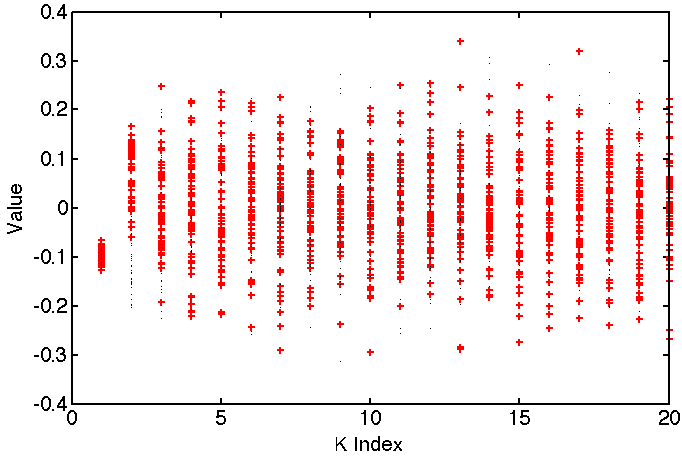
\includegraphics[width=0.7\textwidth]{naive_classifier_k_partition.png}
  \caption{Simple Partitioning: red is male, black is female}
  \label{fig:model:naive:part}
\end{figure}

\pagebreak
\subsection{LDA Classifier} 
\label{sec:model:lda}

Using a training set, we create the matrix $M$ such that each column represents
one image. We then calculate
\[ \left[ U, S, V \right] = \mathrm{svd}(M) \]
and obtain the $V$ coefficients of the remaining data set $M^*$ using
\[ V^* = S \backslash (U \backslash M^*). \]

We did not use all the coefficients in the $V$ matrix, we only used the first
$k$, where $k$ was varied between $5$ and $100$.

We then used MATLAB's \lstinline[language=Matlab]!classify! function, which is
based on Fisher's linear discriminant analysis \cite{classify}. The first $k$
coefficients of $V$ were used as the training set and the first $k$ coefficients
of $V^*$ were to be classified. Because we used the ``diaglinear'' setting,
MATLAB's \lstinline[language=Matlab]!classify! is a na\"ive Bayes classifier.
The setting means that the covariance matrix was diagonal and thus the input
variables are conditionally independent, which means that the classifer is
na\"ive Bayes \cite{nbayes}.

For each $k$ value and training set size, obtaining classification data was
repeated 10 times each with a differently scrambled training set. The accuracies
and false ID percentages shown in the data section are an average of these 10
trials.


\pagebreak
\section{Data And Analysis}
\label{sec:analysis}

In the following section, we present results of our methods used on the FEI
database and the LFW database. It is worth noting that there are 100 males and
100 females in the FEI database, while we used 758 males and 243 females from
the LFW database.

\subsection{Na\"ive Classifier}
\label{sec:analysis:naive}

The na\"ive classifier was only used on the FEI database, on which it yielded
reasonable results. However, we do not believe it to be useful for other images.

The na\"ive classifier was 90\% accurate for the 200 images in the FEI database
and yielded a symmetry of 5\% false identification for both males and females
coincidentally, as seen in Table~\ref{tab:analysis:naive:data}. Looking at the
mean face in Figure~\ref{fig:analysis:naive:mean} for both
male and female faces shows fairly clearly how this classification works
intuitively: Female faces tend to have darker spots next to their necks due to
hair, while male faces have lighter spots. This intuition is confirmed by seeing
that most of the misclassifications are males with long hair and females with
short hair. There are cases in which a misclassification is for another reason,
but the intuition works in most cases.

Because all the faces are seen from a straight angle, we believe that this
classification scheme merely coincidentally worked on the FEI database and would
not work in general.

\begin{table}[!ht]
  \vspace{20pt}
  \centering
  \begin{tabular}{lll}
    \toprule
                      & \bfseries Male  & \bfseries Female  \\
    \bfseries Male    & 45\%            & 5\%               \\
    \bfseries Female  & 5\%             & 45\%              \\
    \bottomrule
  \end{tabular}
  \caption{Results of image classification on FEI database with na\"ive
  classifier}
  \label{tab:analysis:naive:data}
  \vspace{20pt}
\end{table}

\begin{figure}[!ht]
  \centering
  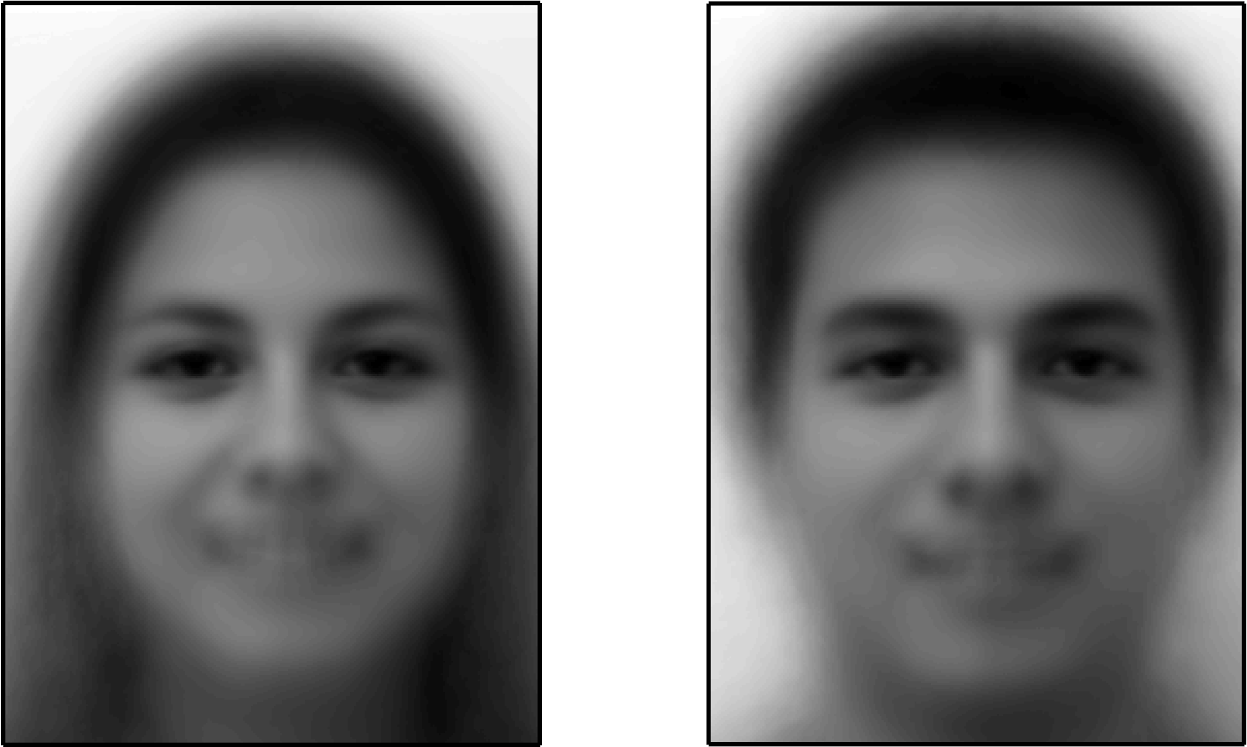
\includegraphics[width=0.7\textwidth]{fei_mean_face_mf.png}
  \caption{FEI mean faces: female on left and male on right.}
  \label{fig:analysis:naive:mean}
\end{figure}

\subsection{LDA Classifier}
\label{sec:analysis:lda}

The LDA classifier performed fairly well when a non-smiling training set was
used on the FEI database. For three cases, its accuracy was 90\% or better; only
the case in which we used gray cropped images and a smiling set was classified
did it perform with 72\% accuracy. This is very likely a result of our method
used: considering the rank-$k$ SVD as a rank-$k$ approximation to the faces, we
note that the difference in images for cropped, gray-scale non-smiling to
cropped, gray-scale smiling is rather large: a smile is now a significant
portion of the face and also much lighter than a non-smiling image in that area.
It stands to reason that feature extraction of the mouth area and usage of the
LDA classifier would also be a good smiling vs non-smiling classifier.

\begin{figure}[!ht]
  \centering
  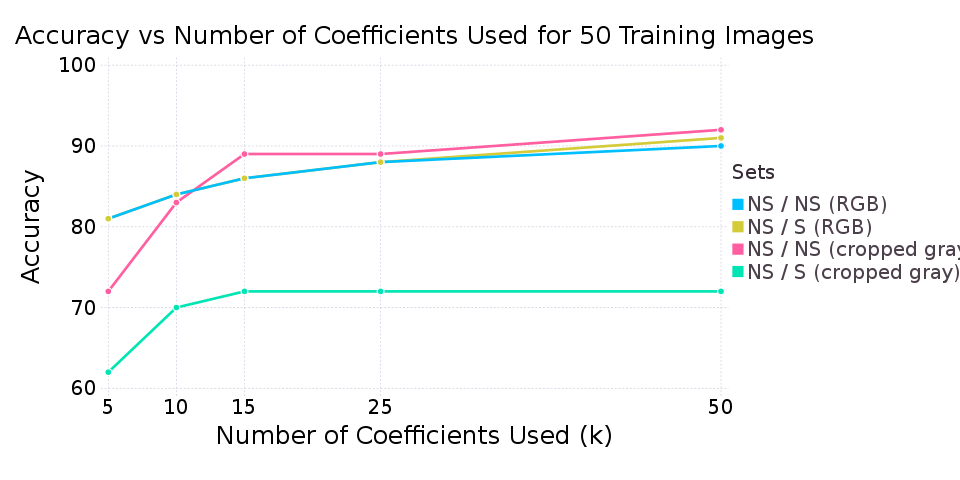
\includegraphics[width=0.8\textwidth]{accuracy_k.png}
  \caption{Accuracy vs number of coefficients used for FEI database when using
  50 images.}
  \label{fig:analysis:lda:accuracy_fei}
\end{figure}

Our data suggests that for the FEI database, $k = 50$ is the optimal number of
coefficients when using $50$ training images as seen in
Figure~\ref{fig:analysis:lda:accuracy_fei}. Appendix~\ref{sec:app:data} also
contains data for using less than $50$ training images with $k$ equal to the
number of training images, but in each case the accuracy is lower than for $k =
50$ with $50$ training images.

For the LFW database, it seems that the highest accuracy we can achieve is about
85.5\%. We used $250$ training images out of a total of $1001$ images and let
$k$ range from $5$ to $100$. Figure~\ref{fig:analysis:lda:mean} shows the mean
faces for all images, male, and female for each color channel (RGB). We notice
that it is hard to tell them apart even for a human and no easy distinction can
be made by looking at the picture as with the na\"ive classifier in
Section~\ref{sec:analysis:naive}. 

\begin{figure}[!ht]
  \centering
  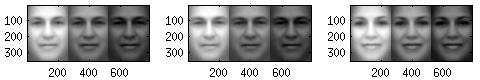
\includegraphics{avg.jpg}
  \caption{LFW mean faces: from left to right; both genders, male, female. Each
  group of three features the red-channel, green-channel, and blue-channel mean
  face. (Axis labels seen are width and height in pixels.)}
  \label{fig:analysis:lda:mean}
\end{figure}

It is to note for the LFW database that the
pictures contained faces at all different angles. This is likely why the mean
faces in Figure~\ref{fig:analysis:lda:mean} look much wider than the average
faces of the FEI database as seen in Figure~\ref{fig:analysis:naive:mean}. This
may also be the reason for the lower overall accuracy. However, if we observe
the accuracy for each gender in Figure~\ref{fig:analysis:lda:accuracy_lfw}, we
note that the female accuracy is much lower than the male accuracy. This is
likely due to the fact that out of $1001$ faces, $758$ were male and $243$ were
female. This means that the training sets likely each had only about
$\nicefrac{1}{4}$ females, which would make it harder to classify female images
accurately. Given an equal amount of male and female images, we hypothesize that
the accuracy of the method on LFW would be similar to the accuracy on FEI.

See all raw data in Appendix~\ref{sec:app:data}.

\begin{figure}[!ht]
  \centering
  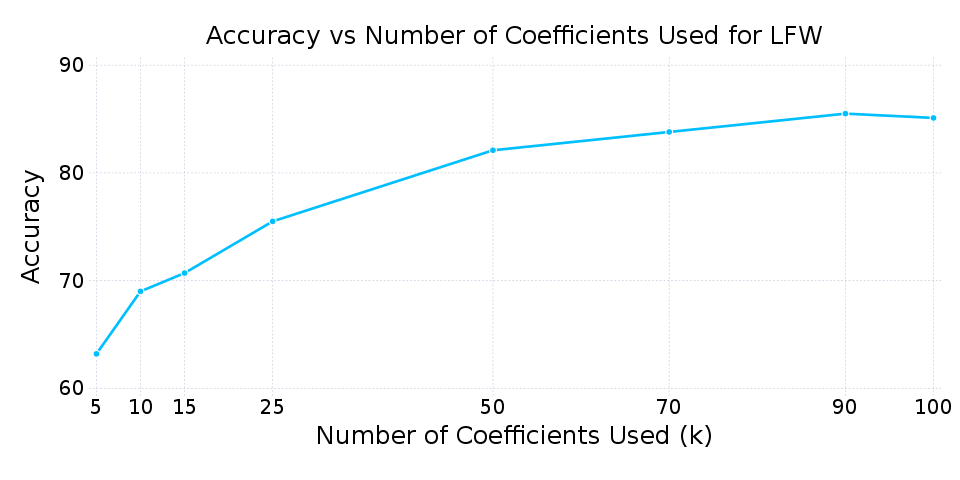
\includegraphics[width=0.8\textwidth]{accuracy_k_lfw.png}
  \caption{Accuracy vs number of coefficients used for Labeled Faces in the
  Wild database.}
  \label{fig:analysis:lda:accuracy_lfw}
\end{figure}

\section{Conclusion}
\label{sec:conclusion}

A na\"ive Bayes classification system such as MATLAB's
\lstinline[language=Matlab]!classify! based on LDA is decent for classifying
gender in both non-smiling and smiling images when a training set of non-smiling
images is used. It seems plausible that such a classifier could also be used to
distinguish other physical characteristics and shapes. 

Even though the images in the Labeled Faces in the Wild were not all from the
same angle, the classifier still achieved up to 85.5\% accuracy when enough
coefficients were used. 

% talk about some future work.

% TODO: 3d surface of k vs training size vs accuracy? -> sunday morning,
% possibly
% TODO: FEI as training set on LFW? -> sunday morning

\pagebreak
\begin{appendices}
  \section{Code}
  \label{sec:app:code}

  \subsection{Classification Algorithm}
  \lstinputlisting[style=c,language=Matlab]{../classifyImages.m}

  \subsection{Image Resizing}
  \subsubsection{crop\_face.py}
  \lstinputlisting[style=c,language=Python]{../crop_face.py}

  \subsubsection{imsize.py}
  \lstinputlisting[style=c,language=Python]{../imsize.py}

  \pagebreak
  \section{Data}
  \label{sec:app:data}

  \begin{longtable}{p{6em} p{5em} p{6em} p{6em} p{6em} p{6em}}
      \toprule
      Training / Classifying & \# training images  & \# coefficient columns  & False ID as M & False
      ID as F & Accuracy \\
      \midrule
      \midrule
      \multirow{3}{6em}{FEI Non-smiling / non-smiling (RGB)} 
                                & 5   & 5   & 39\%  & 38\%  & 61\% \\
                                & 10  & 10  & 26\%  & 21\%  & 75\% \\
                                & 15  & 15  & 19\%  & 15\%  & 81\% \\
                                & 25  & 25  & 13\%  & 14\%  & 87\% \\
                                & 50  & 5   & 20\%  & 18\%  & 81\% \\
                                & 50  & 10  & 18\%  & 15\%  & 84\% \\
                                & 50  & 15  & 15\%  & 14\%  & 86\% \\
                                & 50  & 25  & 12\%  & 13\%  & 88\% \\
                                & 50  & 50  & 8\%   & 10\%  & \bfseries 90\% \\
      \midrule
      \multirow{3}{6em}{FEI Non-smiling / smiling (RGB)} 
                                & 5   & 5   & 15\%  & 22\%  & 80\% \\
                                & 10  & 10  & 17\%  & 16\%  & 81\% \\
                                & 15  & 15  & 13\%  & 14\%  & 86\% \\
                                & 25  & 25  & 11\%  & 13\%  & 88\% \\
                                & 50  & 5   & 9\%   & 14\%  & 88\% \\
                                & 50  & 10  & 11\%  & 13\%  & 88\% \\
                                & 50  & 15  & 12\%  & 12\%  & 88\% \\
                                & 50  & 25  & 11\%  & 11\%  & 89\% \\
                                & 50  & 50  & 11\%  & 9\%   & \bfseries 90\% \\
      \midrule
      \multirow{3}{6em}{FEI Non-smiling / non-smiling (cropped, gray)} 
                                & 5   & 5   & 33\%  & 35\%  & 66\% \\
                                & 10  & 10  & 23\%  & 32\%  & 77\% \\
                                & 15  & 15  & 20\%  & 20\%  & 80\% \\
                                & 25  & 25  & 22\%  & 15\%  & 78\% \\
                                & 50  & 5   & 28\%  & 27\%  & 72\% \\
                                & 50  & 10  & 16\%  & 18\%  & 83\% \\
                                & 50  & 15  & 11\%  & 14\%  & 89\% \\
                                & 50  & 25  & 10\%  & 11\%  & 89\% \\
                                & 50  & 50  & 7\%   & 9\%   & \bfseries 92\% \\
      \midrule
      \multirow{3}{6em}{FEI Non-smiling / smiling (cropped, gray)} 
                                & 5   & 5   & 44\%  & 32\%  & 52\% \\
                                & 10  & 10  & 37\%  & 17\%  & 62\% \\
                                & 15  & 15  & 38\%  & 13\%  & 62\% \\
                                & 25  & 25  & 31\%  & 15\%  & 68\% \\
                                & 50  & 5   & 35\%  & 28\%  & 62\% \\
                                & 50  & 10  & 29\%  & 17\%  & 70\% \\
                                & 50  & 15  & 29\%  & 15\%  & 72\% \\
                                & 50  & 25  & 33\%  & 8\%   & 72\% \\
                                & 50  & 50  & 30\%  & 12\%  & \bfseries 72\% \\
      \midrule
      \multirow{3}{6em}{Labeled Faces in the Wild (cropped, RGB)}
                                & 250 & 5   & 34.6\%  & 43.6\%  & 63.2\% \\
                                & 250 & 10  & 27.1\%  & 43.1\%  & 69\% \\
                                & 250 & 15  & 26.2\%  & 38.8\%  & 70.7\% \\
                                & 250 & 25  & 21.3\%  & 34.3\%  & 75.5\% \\
                                & 250 & 50  & 14.4\%  & 28.6\%  & 82.1\% \\
                                & 250 & 70  & 9.3\%   & 34.8\%  & 83.8\% \\
                                & 250 & 90  & 8.8\%   & 30.7\%  & \bfseries 85.5\% \\
                                & 250 & 100 & 9\%     & 31.7\%  & 85.1\% \\
      \bottomrule
    \caption{Results. Note that there were 758 males and 243 females in the LFW
    database, while there were 100 males and 100 females in the FEI database.}
    \label{tab:data}
  \end{longtable}

\end{appendices}

\pagebreak
\bibliographystyle{amsplain}
\bibliography{proj4}

\end{document}
